\chapter{A Generalized Cost Model for DCJ-Indel Sorting}

%\begin{abstract}
%The double-cut-and-join operation (DCJ) is a fundamental graph operation that is used to model a variety of genome rearrangements.  However, DCJs are only useful when comparing genomes with equal (or nearly equal) gene content.  One obvious extension of the DCJ framework supplements DCJs with insertions and deletions of chromosomes and chromosomal intervals, which implies a model in which DCJs receive unit cost, whereas insertions and deletions receive a nonnegative cost of $\omega$.  This paper proposes a unified model finding a minimum-cost transformation of one genome (with circular chromosomes) into another genome for any value of $\omega$. In the process, it resolves the open case $\omega > 1$.
%\end{abstract}

\section{Preliminaries}
A \textdef{genome} $\Pi$ is a graph containing an even number of labeled nodes and comprising the edge-disjoint union of two perfect matchings: the \textdef{genes}\footnote{In practice, gene edges typically represent synteny blocks containing a large number of contiguous genes} of $\Pi$, denoted $g(\Pi)$; and the \textdef{adjacencies} of $\Pi$, denoted $a(\Pi)$.  Consequently, each node of $\Pi$ has degree 2, and the connected components of $\Pi$ form cycles that alternate between genes and adjacencies; these cycles are called \textdef{chromosomes}.  This genomic model, in which chromosomes are circular, offers a reasonable and commonly used approximation of genomes having linear chromosomes.

A \textdef{double cut and join operation (DCJ)} on $\Pi$, introduced in \cite{yancopoulos}, forms a new genome by replacing two adjacencies of $\Pi$ with two new adjacencies on the same four nodes.  Despite being simply defined, the DCJ incorporates the \textdef{reversal} of a chromosomal segment, the \textdef{fusion} of two chromosomes into one chromosome, and the \textdef{fission} of one chromosome into two chromosomes (Fig.~\ref{figure:DCJ_breakpoint_graph} (top)).\footnote{When the DCJ is applied to circularized linear chromosomes, it encompasses a larger variety of operations. See \cite{braga2010} for details.}  For genomes $\Pi$ and $\Gamma$ with the same genes, the \textdef{DCJ distance}, denoted $d(\Pi, \Gamma)$, is the minimum number of DCJs needed to transform $\Pi$ into $\Gamma$.

The \textdef{breakpoint graph} of $\Pi$ and $\Gamma$, denoted $B(\Pi, \Gamma)$ (introduced in \cite{bafna}), is the edge-disjoint union of $a(\Pi)$ and $a(\Gamma)$ (Fig.~\ref{figure:DCJ_breakpoint_graph} (bottom)).  The line graph of the breakpoint graph is the {\em adjacency graph}, which was introduced in \cite{bergeron} and is also commonly used in genome rearrangement studies.  Note that the connected components of $B(\Pi, \Gamma)$ form cycles (of length at least 2) that alternate between adjacencies of $\Pi$ and $\Gamma$. Letting $c(\Pi, \Gamma)$ denote the number of cycles in $B(\Pi, \Gamma)$, the authors in \cite{yancopoulos} showed that the DCJ distance is given by
\begin{equation}
d(\Pi, \Gamma) = |g(\Pi)| - c(\Pi, \Gamma)\enspace.
\end{equation}

\begin{figure}[h]
\centering
\begin{tabular}{c c}
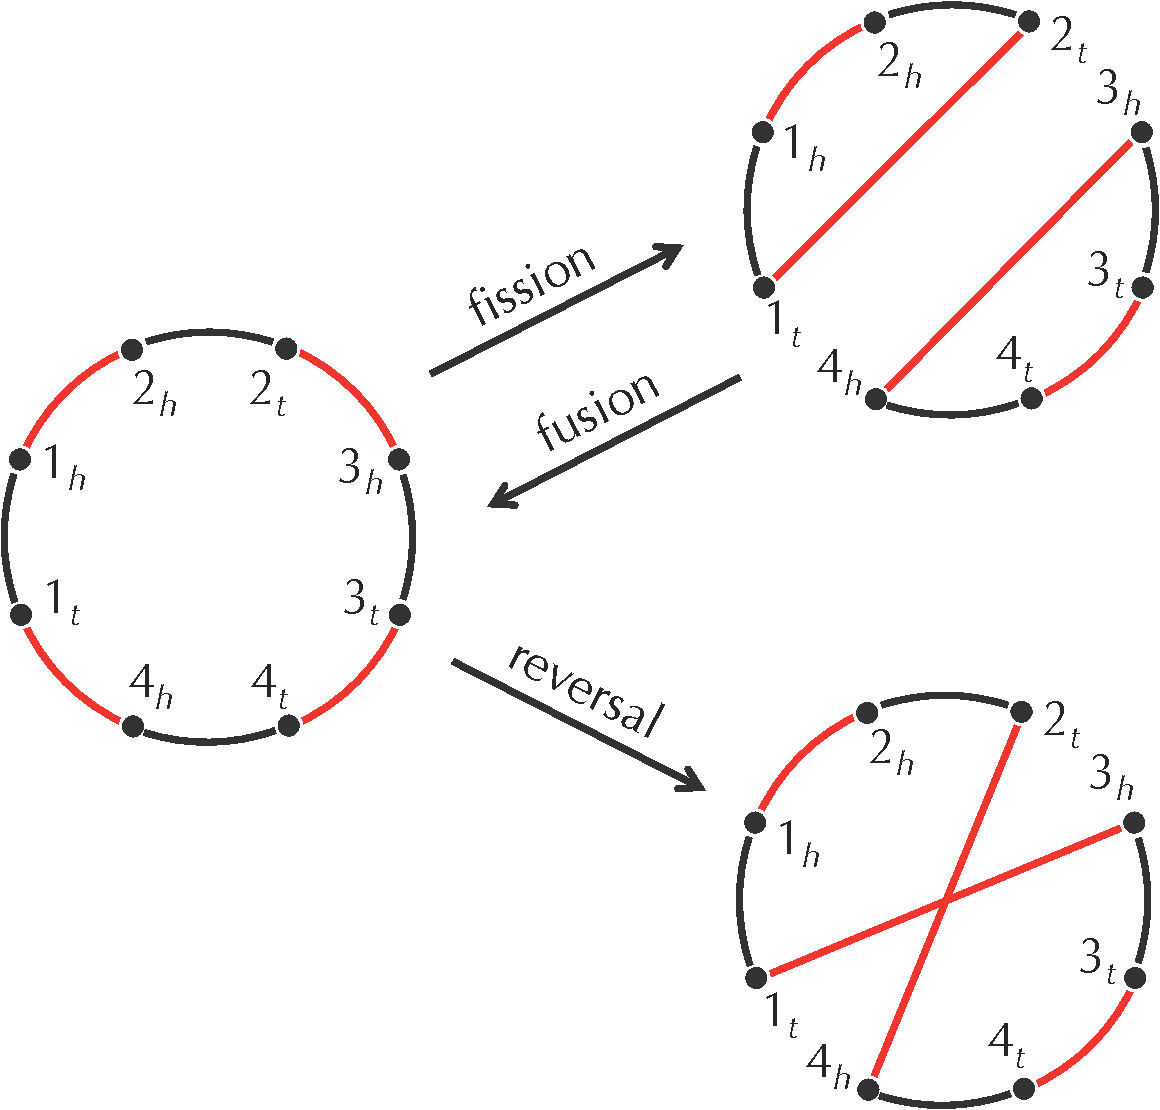
\includegraphics[width = 0.45\textwidth]{images/wabi2014/reversal_fission_and_fusion}\\[5ex]
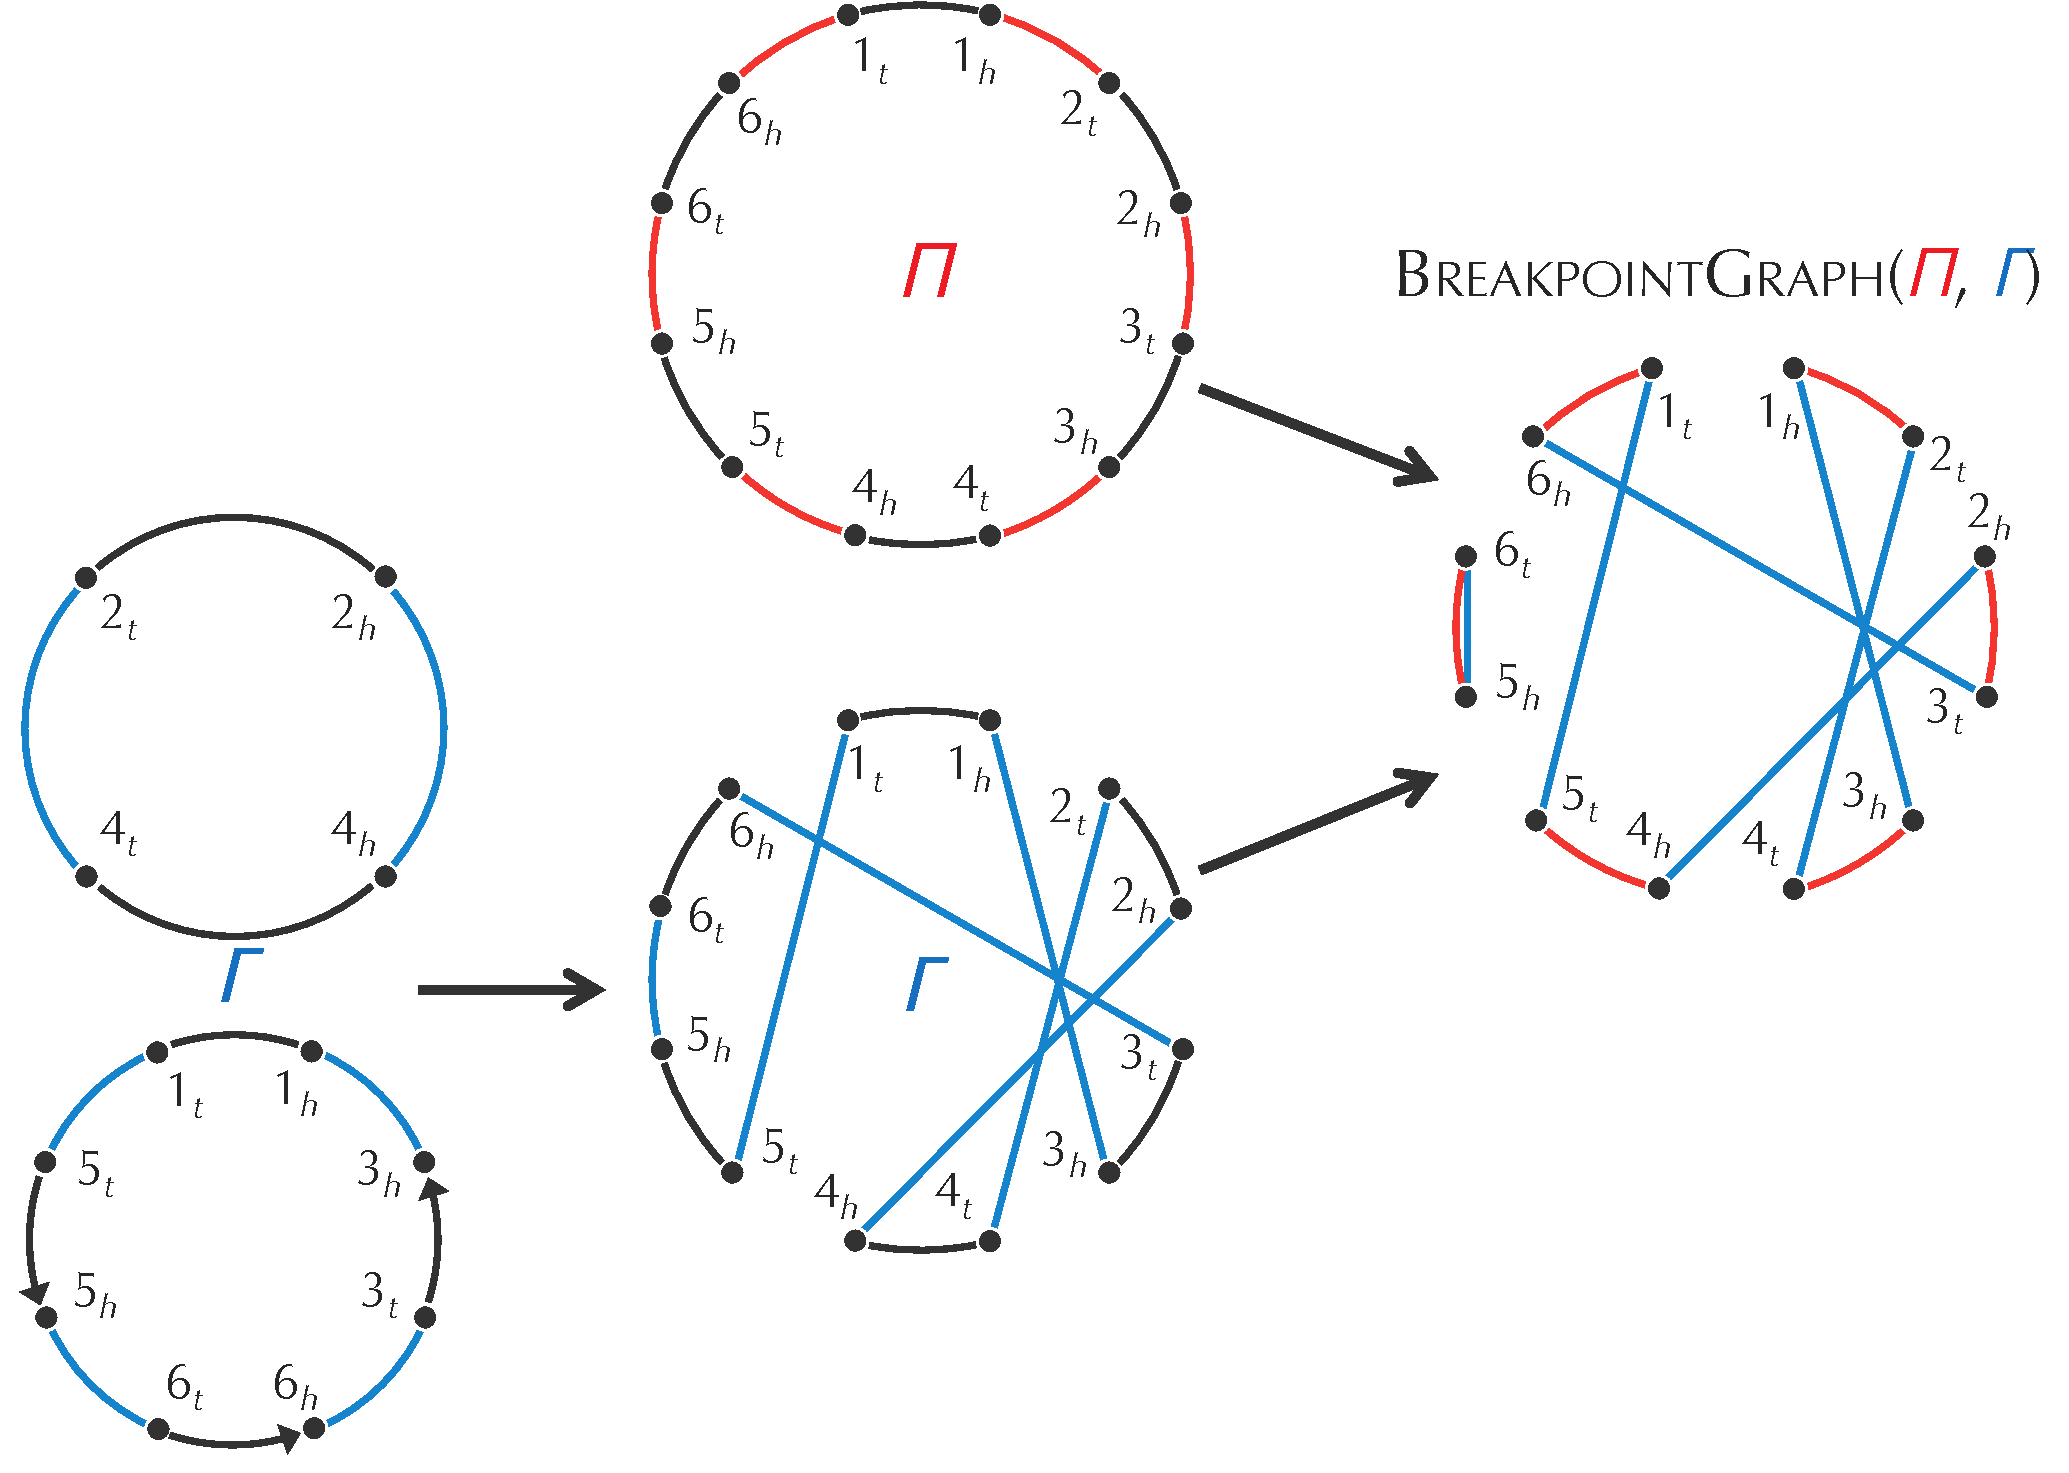
\includegraphics[width = 0.65\textwidth]{images/wabi2014/breakpoint_graph}
\end{tabular}
\label{figure:DCJ_breakpoint_graph}
\caption{(Top) DCJs replace two adjacencies of a genome and incorporate three operations on circular chromosomes: reversals, fissions, and fusions. Genes are shown in black, and adjacencies are shown in red. (Bottom) The construction of the breakpoint graph of genomes $\Pi$ and $\Gamma$ having the same genes. First, the nodes of $\Gamma$ are rearranged so that they have the same position in $\Pi$.  Then, the adjacency graph is formed as the disjoint union of adjacencies of $\Pi$ (red) and $\Gamma$ (blue).}
\end{figure}

The DCJ distance offers a useful metric for measuring the evolutionary distance between two genomes having the same genes, but we strive toward a genomic model that incorporates insertions and deletions as well.  A \textdef{deletion} in $\Pi$ is defined as the removal of either an entire chromosome or chromosomal interval of $\Pi$, i.e., if adjacencies $\{v, w\}$ and $\{x, y\}$ are contained in the order $(v, w, x, y)$ on some chromosome of $\Pi$, then a deletion replaces the path connecting $v$ to $y$ with the single adjacency $\{v, y\}$.  An \textdef{insertion} is simply the inverse operation of a deletion.  The term \textdef{indels} refers collectively to insertions and deletions.

To consider genomes with unequal gene content, we will henceforth assume that any pair of genomes $\Pi$ and $\Gamma$ satisfy $g(\Pi) \cup g(\Gamma) = \mathcal{G}$, where $\mathcal{G}$ is a perfect matching on a collection of nodes $\mathcal{V}$.   A \textdef{transformation} of $\Pi$ into $\Gamma$ is a sequence of DCJs and indels such that any deleted node must belong to $\mathcal{V} - V(\Gamma)$ and any inserted node must belong to $\mathcal{V} - V(\Pi)$.\footnote{This assumption follows the lead of the authors in \cite{braga2010}. It means that we can view any transformation of $\Pi$ into $\Gamma$  prevents, among other things, a trivial transformation of one genome into another genome of similar gene content in which we simply delete all the chromosomes of $\Pi$ and replace them with the chromosomes of $\Gamma$.}

The \textdef{cost} of a transformation $\mathbb{T}$ is equal to the weighted sum of the number of DCJs in $\mathbb{T}$ plus $\omega$ times the number of indels in $\mathbb{T}$, where $\omega$ is some nonnegative constant determined in advance.  The \textdef{DCJ-indel distance} between $\Pi$ and $\Gamma$, denoted $d_{\omega}(\Pi, \Gamma)$, is the minimum cost of any transformation of $\Pi$ into $\Gamma$.  Note that since a transformation of $\Pi$ into $\Gamma$ can be inverted to yield a transformation of $\Gamma$ into $\Pi$, the DCJ-indel distance is symmetric by definition.  Yet unlike the DCJ distance, the DCJ-indel distance does not form a metric, as the triangle inequality does not hold; see \cite{stoye_triangle} for a discussion in the case that $\omega = 1$.

Although we would like to compute DCJ-indel distance, here we are interested in the more difficult problem of \textdef{DCJ-indel sorting}, or producing a minimum cost transformation of $\Pi$ into $\Gamma$.  The case $\omega = 1$ was resolved by the authors in \cite{braga2010}; this result was extended to cover all values $0 \leq \omega \leq 1$ in \cite{braga2012} and \cite{braga2013}.  This work aims to use the simplifying ideas in \cite{compeau2012} and \cite{compeau2013} as a stepping stone for a generalized presentation that will solve the problem of DCJ-indel sorting for all $\omega \geq 0$, thus resolving the open case that $\omega > 1$.

\section{Encoding Indels as DCJs}
A chromosome of $\Pi$ ($\Gamma$) sharing no genes with $\Gamma$ ($\Pi$) is called a \textdef{singleton}.  We use the notation $\mathrm{sing}_{\Gamma}(\Pi)$ to denote the number of singletons of $\Pi$ with respect to $\Gamma$ and the notation $\mathrm{sing}(\Pi, \Gamma)$ to denote the sum $\mathrm{sing}_{\Gamma}(\Pi) + \mathrm{sing}_{\Pi}(\Gamma)$.  We will deal with singletons later; for now, we will show that in the absence of singletons, the insertion or deletion of a chromosomal interval is the only type of indel that we need to consider for the problem of DCJ-indel sorting.

\begin{theorem}
If $\mathrm{sing}(\Pi, \Gamma) = 0$, then any minimum-cost transformation of $\Pi$ into $\Gamma$ cannot include the insertion or deletion of entire chromosomes.
\label{theorem:chromosome_indels}
\end{theorem}

\begin{proof}

We proceed by contradiction.  Say that we have a minimum-cost transformation of $\Pi$ into $\Gamma$ in which (without loss of generality) we are deleting an entire chromosome $C$.  Because $\Pi$ has no singletons, $C$ must have been produced as the result of the deletion of a chromosomal interval or as the result of a DCJ.  $C$ cannot have been produced from the deletion of an interval, since we could have simply deleted the chromosome that $C$ came from. Thus, assuming $C$ was produced as the result of a DCJ, there are now three possibilities:

\begin{enumerate}
\item The DCJ could be a reversal.  In this case, we could have simply deleted the chromosome to which the reversal was appiled, yielding a transformation of strictly smaller cost.
\item The DCJ could be a fission of a chromosome $C'$ that produced $C$ along with another chromosome.  In this case, the genes of $C$ appeared as a contiguous interval of $C'$, which we could have simply deleted at lesser total cost.
\item The DCJ could be the fusion of two chromosomes, $C_1$ and $C_2$.  This case is somewhat more difficult to deal with and is handled by Lemma \ref{lemma:fusion}.
\end{enumerate}

\begin{lemma}
If $\mathrm{sing}_{\Gamma}(\Pi) = 0$, then any minimum-cost transformation of $\Pi$ into $\Gamma$ cannot include the deletion of a chromosome that was produced by a fusion.
\label{lemma:fusion}
\end{lemma}

\begin{proof}
Suppose for the sake of contradiction that a minimum-cost transformation $\mathbb{T}$ of $\Pi$ into $\Gamma$ involves $k$ fusions of $k+1$ chromosomes $C_1, C_2, \ldots, C_{k+1}$ to form a chromosome $C$, which is then deleted.  Without loss of generality, we may assume that this collection of fusions is ``maximal'', i.e., none of the $C_i$ is produced as the result of a fusion.

Because $\Pi$ has no singletons, each $C_i$ must have been produced as a result of a DCJ.  Similar reasoning to that used in the main proof of Theorem \ref{theorem:chromosome_indels} shows that this DCJ cannot be a reversal, and by the assumption of maximality, it cannot be the result of a fusion.  Thus, each $C_i$ is produced by a fission applied to some chromosome $C'_i$ to produce $C_i$ in addition to some other chromosome $C^{*}_i$.

Now, let $\Pi'$ be the genome in $\mathbb{T}$ occurring immediately before these $2k+2$ operations.  Assume that the $k+1$ fissions applied to the $C'_i$ replace adjacencies $\{v_i, w_i\}$ and $\{x_i, y_i\}$ with $\{v_i, y_i\}$ and $\{w_i, x_i\}$.\footnote{It can be verified that these $4k+4$ nodes must be distinct by the assumption that $\mathbb{T}$ has minimum cost.}  Furthermore, assume that the ensuing $k$ fusions are as follows:

\begin{center}
\begin{tabular}{r c l}
$\{v_1, y_1\}, \{v_2, y_2\}$ & $\rightarrow$ & $\{y_1, v_2\}, \{v_1, y_2\}$\\
$\{y_1, v_2\}, \{v_3, y_3\}$  & $\rightarrow$ & $\{y_1, v_3\}, \{v_2, y_3\}$\\
$\{y_1, v_3\}, \{v_4, y_4\}$ & $\rightarrow$ & $\{y_1, v_4\}, \{v_3, y_4\}$\\
& $\vdots$ & \\
$\{y_1, v_k\}, \{v_{k+1}, y_{k+1}\}$ & $\rightarrow$ & $\{y_1, v_{k+1}\}, \{v_k, y_{k+1}\}$
\end{tabular}
\end{center}

The genome resulting from these $2k+1$ operations, which we call $\Pi''_{\mathbb{T}}$, is identical to $\Pi'$ except that for each $i$ ($1 \leq i \leq k+1$), it has replaced the adjacencies $\{v_i, w_i\}$ and $\{x_i, y_i\}$ in $C'_i$ with the adjacencies $\{w_i, x_i\} \in C^{*}_i$ and $\{v_i, y_{i+1 \mod (k+1)}\} \in C$.  In  $\mathbb{T}$, we then delete $C$ from $\Pi''_{\mathbb{T}}$.

Now consider the transformation $\mathbb{U}$ that is identical to $\mathbb{T}$ except that when we reach $\Pi'$, $\mathbb{U}$ first applies the following $k$ DCJs:

\begin{center}
\begin{tabular}{r c l}
$\{v_1, w_1\}, \{x_2, y_2\}$ & $\rightarrow$ & $\{v_1, y_2\}, \{w_1, x_2\}$\\
$\{v_2, w_2\}, \{x_3, y_3\}$ & $\rightarrow$ & $\{v_2, y_3\}, \{w_2, x_3\}$\\
$\{v_3, w_3\}, \{x_4, y_4\}$ & $\rightarrow$ & $\{v_3, y_4\}, \{w_3, x_4\}$\\
& $\vdots$ & \\
$\{v_k, w_k\}, \{x_{k+1}, y_{k+1}\}$ & $\rightarrow$ & $\{v_k, y_{k+1}\}, \{w_k, x_{k+1}\}$
\end{tabular}
\end{center}

\noindent $\mathbb{U}$ then applies $k$ subsequent DCJs as follows:

\begin{center}
\begin{tabular}{r c l}
$\{x_1, y_1\}, \{w_1, x_2\}$ &  $\rightarrow$ & $\{y_1, x_2\}, \{w_1, x_1\}$\\
$\{y_1, x_2\}, \{w_2, x_3\}$ &  $\rightarrow$ & $\{y_1, x_3\}, \{w_2, x_2\}$\\
$\{y_1, x_3\}, \{w_3, x_4\}$ & $\rightarrow$ & $\{y_1, x_4\}, \{w_3, x_3\}$\\
& $\vdots$ & \\
$\{y_1, x_k\}, \{w_k, x_{k+1}\}$ & $\rightarrow$ & $\{y_1, x_{k+1}\}, \{w_k, x_k\}$
\end{tabular}
\end{center}

The resulting genome, which we call $\Pi''_{\mathbb{U}}$, has the exact same adjacencies as $\Pi''_{\mathbb{T}}$ except that it contains the adjacencies $\{y_1, x_{k+1}\}$ and $\{v_{k+1}, w_{k+1}\}$ instead of $\{v_{k+1}, y_1\}$ and $\{w_{k+1}, x_{k+1}\}$.  Because two genomes on the same genes are equivalent if and only if they share the same adjacencies, a single DCJ on $\{y_1, x_{k+1}\}$ and $\{v_{k+1}, w_{k+1}\}$ would change $\Pi''_{\mathbb{U}}$ into $\Pi''_{\mathbb{T}}$.  Furthermore, in $\Pi''_{\mathbb{T}}$, $\{v_{k+1}, y_1\}$ belongs to $C$ and $\{w_{k+1}, x_{k+1}\}$ belongs to $C^{*}_{k+1}$, so that this DCJ in question must be a fission producing $C$ and $C^{*}_{k+1}$. In $\mathbb{U}$, rather than applying this fission, we simply delete the chromosomal interval containing the genes of $C$. As a result, $\mathbb{U}$ is identical to $\mathbb{T}$ except that it replaces $2k + 1$ DCJs and a deletion by $2k$ DCJs and a deletion. Hence, $\mathbb{U}$ has strictly smaller cost than $\mathbb{T}$, which provides the desired contradiction.
\end{proof}
\end{proof}

\noindent Following Theorem \ref{theorem:chromosome_indels}, we recall the observation in \cite{arndt} that we can view the deletion of a chromosomal interval replacing adjacencies $\{v, w\}$ and $\{x, y\}$ with the single adjacency as a fission replacing $\{v, w\}$ and $\{x, y\}$ by the two adjacencies $\{w, x\}$ and $\{v, y\}$, thus forming a circular chromosome containing $\{v, y\}$ that is scheduled for later removal. By viewing this operation as a DCJ, we establish a bijective correspondence between the deletions of a minimum cost transformation of $\Pi$ into $\Gamma$ (having no singletons) and a collection of chromosomes sharing no genes with $\Pi$.  (Insertions are handled symmetrically.)

Therefore, define a \textdef{completion} of genomes $\Pi$ and $\Gamma$ as a pair of genomes $(\Pi', \Gamma')$ such that $\Pi$ is a subgraph of $\Pi'$, $\Gamma$ is a subgraph of $\Gamma'$, and $g(\Pi') = g(\Gamma') = \mathcal{G}$.  Each of $\Pi' - \Pi$ and $\Gamma' - \Gamma$ is formed of alternating cycles called \textdef{new chromosomes}; by our bijective correspondence, we use $\mathrm{ind}(\Pi', \Gamma')$ to denote the total number of new chromosomes of $\Pi'$ and $\Gamma'$.   We will amortize the cost of a deletion by charging unit cost for the DCJ that produces a new chromosome, followed by $1 - \omega$ for the removal of this chromosome, yielding our next result.  For simplicity, we henceforth set $N = |\mathcal{V}|/2$, the number of genes of $\Pi$ and $\Gamma$.

\begin{theorem}
If $\mathrm{sing}(\Pi, \Gamma) = 0$, then
\begin{align}
d_{\omega}(\Pi, \Gamma) & = \min_{(\Pi', \Gamma')}{\{d(\Pi', \Gamma') + (\omega - 1)\cdot \mathrm{ind}(\Pi', \Gamma')\}} \label{equation:DCJ-indel_min} \\
 & = N - \max_{(\Pi', \Gamma')}{\{c(\Pi', \Gamma') + (1 - \omega)\cdot \mathrm{ind}(\Pi', \Gamma')\}} \label{equation:DCJ-indel_max}
\end{align}
where the optimization is taken over all completions of $\Pi$ and $\Gamma$. 
\label{theorem:DCJ-indel_optimization}
\end{theorem}

\noindent A completion $(\Pi^{*}, \Gamma^{*})$ is called \textdef{optimal} if it achieves the maximum in (\ref{equation:DCJ-indel_max}).  We plan to use Theorem \ref{theorem:DCJ-indel_optimization} to construct an optimal completion for genomes lacking singletons.  Once we have formed an optimal completion $(\Pi^*, \Gamma^*)$, we can simply invoke the $O(N)$-time sorting algorithm described in \cite{bergeron} to transform $\Pi^*$ into $\Gamma^*$ via a minimum collection of DCJs.

\section{DCJ-Indel Sorting Genomes without Singletons}

Define a node $v \in \mathcal{V}$ to be $\mathbf{\Pi}$\textbf{-open} ($\mathbf{\Gamma}$\textbf{-open}) if $v \notin \Pi$ ($v \notin \Gamma$).  When forming adjacencies of $\Pi^{*}$ ($\Gamma^{*}$), we connect pairs of $\Pi$-open ($\Gamma$-open) nodes.   Given genomes $\Pi$ and $\Gamma$ with unequal gene content, we can still define the breakpoint graph $B(\Pi, \Gamma)$ as the edge-disjoint union of $a(\Pi)$ and $a(\Gamma)$; however, because the adjacencies of $\Pi$ and $\Gamma$ are not necessarily perfect matchings on $\mathcal{V}$, $B(\Pi, \Gamma)$ may contain paths (of positive length) in addition to cycles.  

We can view the problem of constructing an optimal completion $(\Pi^*, \Gamma^*)$ as adding edges to  $B(\Pi, \Gamma)$ to form $B(\Pi^*, \Gamma^*)$.  Our hope is to construct these edges via direct analysis of $B(\Pi, \Gamma)$.  First, note that cycles of $B(\Pi, \Gamma)$ must embed as cycles of $B(\Pi^*, \Gamma^*)$, whereas odd-length paths of $B(\Pi, \Gamma)$ end in either two $\Pi$-open nodes or two $\Gamma$-open nodes, and even-length paths of $B(\Pi, \Gamma)$ end in a $\Pi$-open node and a $\Gamma$-open node.  The paths of $B(\Pi, \Gamma)$ must be \textdef{linked} in some way by edges in $a(\Pi^{*}) - a(\Pi)$ or $a(\Gamma^{*}) - a(\Gamma)$ to form cycles alternating between edges of $a(\Pi^{*})$ and $a(\Gamma^{*})$. Our basic intuition is to do so in such a way as to create as many cycles as possible, at least when $\omega$ is small; this intuition is confirmed by the following two results.

\begin{proposition}
If $0 < \omega < 2$ and $\mathrm{sing}(\Pi, \Gamma) = 0$, then for any optimal completion $(\Pi^*, \Gamma^*)$ of $\Pi$ and $\Gamma$, every path of length $2k-1$ in $B(\Pi, \Gamma)$ $(k \geq 1)$ embeds into a cycle of length $2k$ in $B(\Pi^*, \Gamma^*)$.
\label{proposition:odd_paths}
\end{proposition}

\begin{proof}
Let $P$ be a path of length $2k-1$ in $B(\Pi, \Gamma)$. Without loss of generality, assume that $P$ has $\Pi$-open nodes $v$ and $w$ as endpoints. Suppose that for some completion $(\Pi', \Gamma')$, $P$ does not embed into a cycle of length $2k$ in $B(\Pi', \Gamma')$ (i.e., $\{v, w\}$ is not an adjacency of $\Pi'$); in this case, we must have distinct adjacencies $\{v, x\}$ and $\{w, y\}$ in $\Pi'$ belonging to the same cycle of $B(\Pi, \Gamma)$.

Consider the completion $\Pi''$ that is formed from $\Pi'$ by replacing $\{v, x\}$ and $\{w, y\}$ with $\{v, w\}$ and $\{x, y\}$.  It is clear that $c(\Pi'', \Gamma') = c(\Pi', \Gamma') + 1$ and $|\mathrm{ind}(\Pi'', \Gamma') - \mathrm{ind}(\Pi', \Gamma')| < 1$.  Thus, it follows from (\ref{equation:DCJ-indel_max}) that $(\Pi', \Gamma')$ cannot be optimal. 
\end{proof}

\noindent As a result of Proposition \ref{proposition:odd_paths}, when $0 < \omega < 2$, any cycle of $B(\Pi^{*}, \Gamma^{*})$ that is not induced from a cycle or odd-length path of $B(\Pi, \Gamma)$ must be a \textdef{\textit{k}-bracelet}, which contains $k$ even-length paths of $B(\Pi, \Gamma)$, where $k$ is even.  We use the term \textdef{bracelet links} to refer to adjacencies of a bracelet belonging to new chromosomes; each $k$-bracelet in $B(\Pi^{*}, \Gamma^{*})$ contains $k/2$ bracelet links from $\Pi^{*} - \Pi$ and $k/2$ bracelet links from $\Gamma^{*} - \Gamma$.  According to (\ref{equation:DCJ-indel_max}), we need to make $c(\Pi^{*}, \Gamma^{*})$ large, which means that when indels are inexpensive, we should have bracelets containing as few bracelet links as possible.

\begin{proposition}
If $0 < \omega < 2$ and $\mathrm{sing}(\Pi, \Gamma) = 0$, then for any optimal completion $(\Pi^*, \Gamma^*)$ of $\Pi$ and $\Gamma$, all of the even-length paths of $B(\Pi, \Gamma)$ embed into 2-bracelets of $B(\Pi^*, \Gamma^*)$.
\label{proposition:even_paths}
\end{proposition}

\begin{proof}
Suppose that a completion $(\Pi', \Gamma')$ of $\Pi$ and $\Gamma$ contains a $k$-bracelet for $k \geq 4$.  This bracelet must contain two bracelet adjacencies $\{v, w\}$ and $\{x, y\}$ belonging to $a(\Pi')$, where these four nodes are contained in the order $(v, w, x, y)$ in the bracelet. Consider the genome $\Pi''$ that is obtained from $\Pi'$ by replacing $\{v, w\}$ and $\{x, y\}$ with $\{v,y\}$ and $\{w, x\}$.  As in the proof of Proposition \ref{proposition:odd_paths}, $c(\Pi'', \Gamma') = c(\Pi', \Gamma') + 1$ and $|\mathrm{ind}(\Pi'', \Gamma') - \mathrm{ind}(\Pi', \Gamma')| < 1$, so that $(\Pi', \Gamma')$ cannot be optimal.
\end{proof}

\noindent The conditions provided by the previous two propositions are very strong. To resolve the case that $0 < \omega < 2$, note that if we must link the endpoints of any odd-length path in $B(\Pi, \Gamma)$ to construct an optimal completion, then we may first create some new chromosomes before dealing with the case of even-length paths.  Let $k_{\Gamma}(\Pi)$ be the number of new chromosomes formed by linking the endpoints of odd-length paths of $B(\Pi, \Gamma)$ that end with $\Pi$-open nodes, and set $k(\Pi, \Gamma) = k_{\Gamma}(\Pi) + k_{\Pi}(\Gamma)$.  After linking the endpoints of odd-length paths, if we can link pairs of even-length paths (assuming any exist) into 2-bracelets so that one \emph{additional} new chromosome is created in each of $\Pi^{*}$ and $\Gamma^{*}$, then we will have constructed an optimal completion.  This construction is guaranteed by the following proposition.

\begin{proposition}
If $0 < \omega < 2$ and $\mathrm{sing}(\Pi, \Gamma) = 0$, then any optimal completion $(\Pi^*, \Gamma^*)$ of $\Pi$ and $\Gamma$ has the property that one new chromosome of $\Pi^{*}$ $(\Gamma^{*})$ contains all of the bracelet adjacencies of $\Pi^{*}$ $(\Gamma^{*})$.
\end{proposition}

\begin{proof}
By Proposition \ref{proposition:odd_paths}, we may assume that we have started forming an optimal completion $(\Pi^{*}, \Gamma^{*})$ by linking the endpoints of any odd-length paths in $B(\Pi, \Gamma)$ to each other.  Given any even-length path $P$ in $B(\Pi, \Gamma)$, there is exactly one other even-length path $P_1$ that would form a new chromosome in $\Gamma^{*}$ if linked with $P$, and exactly one other even-length path $P_2$ in $B(\Pi, \Gamma)$ that would form a new chromosome in $\Pi^{*}$ if linked with $P$ ($P_1$ and $P_2$ may be the same).  As long as there are more than two other even-length paths to choose from, we can simply link $P$ to any path other than $P_1$ or $P_2$. We then iterate this process until two even-length paths remain, which we link to complete the construction of $\Pi^{*}$ and $\Gamma^{*}$; each of these genomes has  one new chromosome containing all of that genome's bracelet adjacencies.
\end{proof}

\noindent It is easy to see that the conditions in the preceding three propositions are sufficient (but not necessary) when constructing an optimal completion for the boundary cases $\omega = 0$ and $\omega = 2$.  We are now ready to state our first major result with respect to DCJ-indel sorting.

\begin{algorithm}
When $0 \leq \omega \leq 2$ and $\mathrm{sing}(\Pi, \Gamma) = 0$, the following algorithm solves the problem of DCJ-indel sorting $\Pi$ into $\Gamma$ in $O(N)$ time.
\begin{enumerate}
\item Link the endpoints of any odd-length path in $B(\Pi, \Gamma)$, which may create some new chromosomes in $\Pi^{*}$ and $\Gamma^{*}$.
\item Arbitrarily select an even-length path $P$ of $B(\Pi, \Gamma)$ (if one exists).
\begin{enumerate}
\item If there is more than one additional even-length path in $B(\Pi, \Gamma)$, link $P$ to an even-length path that produces no new chromosomes in $\Pi^{*}$ or $\Gamma^{*}$.
\item Otherwise, link the two remaining even-length paths in $B(\Pi, \Gamma)$ to form a new chromosome in each of $\Pi^{*}$ and $\Gamma^{*}$.
\end{enumerate}
\item Iterate Step 2 until no even-length paths of $B(\Pi, \Gamma)$ remain. The resulting completion is $(\Pi^{*}, \Gamma^{*})$.
\item Apply the $O(N)$-time algorithm for DCJ sorting from \cite{yancopoulos} to transform $\Pi^{*}$ into $\Gamma^{*}$.
\end{enumerate}
\label{algorithm:small_omega}
\end{algorithm}

\noindent Let $p_{\mathrm{odd}}(\Pi, \Gamma)$ and $p_{\mathrm{even}}(\Pi, \Gamma)$ equal the number of odd- and even-length paths in $B(\Pi, \Gamma)$, respectively.  The optimal completion $(\Pi^{*}, \Gamma^{*})$ constructed by Algorithm \ref{algorithm:small_omega} has the following properties:
\begin{align}
c(\Pi^{*}, \Gamma^{*}) & = c(\Pi, \Gamma) + p_{\mathrm{odd}}(\Pi, \Gamma) + \dfrac{p_{\mathrm{even}}(\Pi, \Gamma)}{2} \label{equation:small_omega_optimal_completion_cycles} \\
\mathrm{ind}(\Pi^{*}, \Gamma^{*}) & = k(\Pi, \Gamma) + \min{\{2, p_{\mathrm{even}}(\Pi, \Gamma)\}} \label{equation:small_omega_optimal_completion_indels}
\end{align}

\noindent These formulas, when combined with Theorem \ref{theorem:DCJ-indel_optimization}, yield a formula for the DCJ-indel distance as a function of $\Pi$, $\Gamma$, and $\omega$ alone.

\begin{corollary}
If $0 \leq \omega \leq 2$ and $\mathrm{sing}(\Pi, \Gamma) = 0$, the DCJ-indel distance between $\Pi$ and $\Gamma$ is given by the following equation:
\begin{equation}
\begin{split}
d_{\omega}(\Pi, \Gamma) = N - & \bigg[ \Big(c(\Pi, \Gamma) + p_{\mathrm{odd}}(\Pi, \Gamma) + \frac{p_{\mathrm{even}}(\Pi, \Gamma)}{2}\Big) + \Big(1 - \omega\Big) \cdot  \\
&  \phantom{[} \Big(k(\Pi, \Gamma) + \min{\big\{2, p_{\mathrm{even}}(\Pi, \Gamma)\big\}}\Big) \bigg]
\end{split}
\label{equation:small_omega_distance}
\end{equation}
\label{corollary:small_omega_distance}
\end{corollary}

\noindent We now turn our attention to the case $\omega > 2$.  Intuitively, as $\omega$ grows, we should witness fewer indels. Let $\delta_{\Gamma}(\Pi)$ be equal to 1 if $g(\Pi) - g(\Gamma)$ is nonempty and 0 otherwise; then, set $\delta(\Pi, \Gamma) = \delta_{\Gamma}(\Pi) + \delta_{\Pi}(\Gamma)$.  Note that $\delta(\Pi, \Gamma)$ is a lower bound on the number of indels in any transformation of $\Pi$ into $\Gamma$.  The following result shows that in the absence of singletons, this bound is achieved by every minimum-cost transformation when $\omega > 2$.

\begin{theorem}
If $\omega > 2$ and $\mathrm{sing}(\Pi, \Gamma) = 0$, then any minimum-cost transformation of $\Pi$ into $\Gamma$ has at most insertion and at most one deletion. As a result,
\begin{equation}
d_{\omega}(\Pi, \Gamma) = N - \max_{\mathrm{ind}(\Pi', \Gamma') = \delta(\Pi, \Gamma)}{\{c(\Pi', \Gamma') + (1 - \omega) \cdot \delta(\Pi, \Gamma)\}}\enspace.
\label{equation:one_indel}
\end{equation}
\label{theorem:one_indel}
\end{theorem}
\vspace{-1.5\baselineskip}

\begin{proof}
Suppose for the sake of contradiction that $\mathbb{T}$ is a minimum-cost transformation of $\Pi$ into $\Gamma$ and that (without loss of generality) $\mathbb{T}$ contains two deletions of chromosomal intervals $P_1$ and $P_2$, costing $2\omega$.  Say that one of these deletions replaces adjacencies $\{v, w\}$ and $\{x, y\}$ with $\{v, y\}$ (deleting the interval connecting $w$ to $x$)  and the other deletion replaces adjacencies $\{a, b\}$ and $\{c, d\}$ with $\{a, d\}$ (deleting the interval connecting $b$ to $c$).

Consider a second transformation $\mathbb{U}$ that is otherwise identical to $\mathbb{T}$, except that it replaces the deletions of $P_1$ and $P_2$ with three operations.  First, a DCJ replaces $\{v, w\}$ and $\{a, b\}$ with $\{v, a\}$ and $\{w, b\}$; the new adjacency $\{w, b\}$ joins $P_1$ and $P_2$ into a single chromosomal interval $P$.  Second, a deletion removes $P$ and replaces adjacencies $\{c, d\}$ and $\{x, y\}$ with the single adjacency $\{d, y\}$.  Third, another DCJ replaces $\{v, a\}$ and $\{d, y\}$ with the adjacencies $\{v, y\}$ and $\{a, d\}$, yielding the same genome as the first scenario at a cost of $2 + \omega$.  Because $\mathbb{U}$ is otherwise the same as $\mathbb{T}$, $\mathbb{U}$ will have strictly lower cost precisely when $\omega > 2$, in which case $\mathbb{T}$ cannot have minimum cost.
\end{proof}

\noindent One can verify that the condition in Theorem \ref{theorem:one_indel} is sufficient but not necessary to guarantee a minimum-cost transformation when $\omega = 2$.  Furthermore, a consequence of Theorem \ref{theorem:one_indel} is that the optimal completion is independent of the value of $\omega$.  In other words, if a completion achieves the maximum in (\ref{equation:one_indel}), then this completion is automatically optimal for \emph{all} values of $\omega \geq 2$.

Fortunately, Algorithm \ref{algorithm:small_omega} already describes the construction of a completion $(\Pi', \Gamma')$ that is optimal when $\omega = 2$.  Of course, we cannot guarantee that this completion has the desired property that $\mathrm{ind}(\Pi', \Gamma') = \delta(\Pi, \Gamma)$.  However, if $\mathrm{ind}(\Pi', \Gamma') > \delta(\Pi, \Gamma)$, then we can apply $\mathrm{ind}(\Pi', \Gamma') - \delta(\Pi, \Gamma)$ total fusions to $\Pi'$ and $\Gamma'$ in order to obtain a different completion $(\Pi^{*}, \Gamma^{*})$.  Each of these fusions reduces the number of new chromosomes by 1 and (by (\ref{equation:DCJ-indel_max})) must also decrease the number of cycles in the breakpoint graph by 1, since $(\Pi', \Gamma')$ is optimal for $\omega = 2$. As a result, $c(\Pi^{*}, \Gamma^{*}) - \mathrm{ind}(\Pi^{*}, \Gamma^{*}) = c(\Pi', \Gamma') - \mathrm{ind}(\Pi', \Gamma')$.  Thus, $(\Pi^{*}, \Gamma^{*})$ is optimal for $\omega = 2$, and since $\mathrm{ind}(\Pi^{*}, \Gamma^{*}) = \delta(\Pi, \Gamma)$, we know that $(\Pi^{*}, \Gamma^{*})$ must be optimal for any $\omega > 2$ as already noted.  This discussion immediately implies the following algorithm.

\begin{algorithm}
If $\omega \geq 2$ and $\mathrm{sing}(\Pi, \Gamma) = 0$, then the following algorithm solves the problem of DCJ-indel sorting $\Pi$ into $\Gamma$ in $O(N)$ time.
\begin{enumerate}
\item Follow the first three steps of Algorithm \ref{algorithm:small_omega} to construct a completion $(\Pi', \Gamma')$ that is optimal for $\omega = 2$.
\item Apply a total of $\mathrm{ind}(\Pi', \Gamma') - \delta(\Pi, \Gamma)$ fusions to $\Pi'$ and $\Gamma'$ in order to produce a completion $(\Pi^{*}, \Gamma^{*})$ having $\mathrm{ind}(\Pi^{*}, \Gamma^{*}) = \delta(\Pi, \Gamma)$.
\item Apply the $O(N)$-time algorithm for DCJ sorting from \cite{yancopoulos} to transform $\Pi^{*}$ into $\Gamma^{*}$.  Any DCJ involving a new chromosome can be viewed as an indel.
\end{enumerate}
\label{algorithm:large_omega}
\end{algorithm}

\noindent The optimal completion $(\Pi^{*}, \Gamma^{*})$ returned by Algorithm \ref{algorithm:large_omega} has the property that
\begin{equation}
c(\Pi^{*}, \Gamma^{*}) = c(\Pi, \Gamma) + p_{\mathrm{odd}}(\Pi, \Gamma) + \dfrac{p_{\mathrm{even}}(\Pi, \Gamma)}{2} - \Big[\mathrm{ind}(\Pi', \Gamma') - \delta(\Pi, \Gamma)\Big]\enspace,
\label{equation:optimal_completion_large_omega}
\end{equation}
\noindent where $(\Pi', \Gamma')$ is the optimal completion for $\omega = 2$ returned by Algorithm \ref{algorithm:small_omega}.  Combining this equation with (\ref{equation:small_omega_optimal_completion_indels}) and (\ref{equation:one_indel}) yields a closed formula for the DCJ-indel distance when $\omega > 2$ in the absence of singletons.

\begin{corollary}
If $\omega \geq 2$ and $\mathrm{sing}(\Pi, \Gamma) = 0$, then the DCJ-indel distance between $\Pi$ and $\Gamma$ is given by the following equation:
\begin{equation}
\begin{split}
d_{\omega}(\Pi, \Gamma) = N -  \bigg[ \Big( & c(\Pi, \Gamma) + p_{\mathrm{odd}}(\Pi, \Gamma) + \frac{p_{\mathrm{even}}(\Pi, \Gamma)}{2} - k(\Pi, \Gamma) - \phantom{x} \\
& \min{\big\{2, p_{\mathrm{even}}(\Pi, \Gamma)\big\}}\Big) +  (2 - \omega) \cdot \delta(\Pi, \Gamma)\bigg]
\end{split}
\label{equation:large_omega_distance}
\end{equation}
\label{corollary:large_omega_distance}
\end{corollary}
\vspace{-\baselineskip}

\section{Incorporating Singletons into DCJ-Indel Sorting}

We have thus far avoided genome pairs with singletons because Theorem \ref{theorem:chromosome_indels}, which underlies the main results in the preceding section, only applied in the absence of singletons. Yet fortunately, genomes with singletons will be relatively easy to incorporate into a single DCJ-indel sorting algorithm. As we might guess, different values of $\omega$ produce different results.

\begin{theorem}
If $\Pi^{\emptyset}$ and $\Gamma^{\emptyset}$ are produced from genomes $\Pi$ and $\Gamma$ by removing all singletons, then
\begin{equation}
\begin{split}
d_{\omega}(\Pi, \Gamma) = & d_{\omega}(\Pi^{\emptyset}, \Gamma^{\emptyset}) + \min{\{1, \omega\}} \cdot \mathrm{sing}(\Pi, \Gamma) + \max{\{0, \omega - 1\}} \cdot\\
& \Big[ (1 - \delta_{\Gamma^{\emptyset}}(\Pi^{\emptyset}))\cdot \min{\{1, \mathrm{sing}_{\Gamma}(\Pi)\}} + \\
&\phantom{(} (1 - \delta_{\Pi^{\emptyset}}(\Gamma^{\emptyset})) \cdot \min{\{1, \mathrm{sing}_{\Pi}(\Gamma)\}}\Big]
\end{split}
\label{equation:singletons}
\end{equation}
\end{theorem}
\vspace{-\baselineskip}

\begin{proof}
Any transformation of $\Pi^{\emptyset}$ into $\Gamma^{\emptyset}$ can be supplemented by the deletion of each singleton of $\Pi$ and the insertion of each singleton of $\Gamma$ to yield a collection of DCJs and indels transforming $\Pi$ into $\Gamma$.  As a result, for any value of $\omega$,
\begin{equation}
d_{\omega}(\Pi, \Gamma) \leq d_{\omega}(\Pi^{\emptyset}, \Gamma^{\emptyset}) + \omega \cdot \mathrm{sing}(\Pi, \Gamma)\enspace.
\label{equation:singleton_upper_bound}
\end{equation}

Next, we will view an arbitrary transformation $\mathbb{T}$ of $\Pi$ into $\Gamma$ as a sequence $(\Pi_0, \Pi_1, \ldots, \Pi_n)$ ($n \geq 1$), where $\Pi_0 = \Pi$, $\Pi_n = \Gamma$, and $\Pi_{i+1}$ is obtained from $\Pi_i$ as the result of a single DCJ or indel. Consider a sequence $(\Pi^{\emptyset}_0, \Pi^{\emptyset}_1, \ldots, \Pi^{\emptyset}_n)$, where $\Pi^{\emptyset}_i$ is constructed from $\Pi_i$ by removing the subgraph of $\Pi_i$ induced by the nodes of the singletons of $\Pi$ and $\Gamma$ under the stipulation that whenever we remove a path $P$ connecting $v$ to $w$, we replace adjacencies $\{v, x\}$ and $\{w, y\}$ in $\Pi_i$ with $\{x, y\}$ in $\Pi^{\emptyset}_i$.  Certainly, $\Pi^{\emptyset}_0 = \Pi^{\emptyset}$ and $\Pi^{\emptyset}_n = \Gamma^{\emptyset}$. Furthermore, for every $i$ in range, if $\Pi^{\emptyset}_{i+1}$ is not the result of a DCJ or indel applied to $\Pi^{\emptyset}_i$, then $\Pi^{\emptyset}_{i+1} = \Pi^{\emptyset}_i$. Thus, $(\Pi^{\emptyset}_0, \Pi^{\emptyset}_1, \ldots, \Pi^{\emptyset}_n)$ can be viewed as encoding a transformation of $\Pi^{\emptyset}$ into $\Gamma$ using \emph{at most} $n$ DCJs and indels.  One can verify that $\Pi^{\emptyset}_{i+1} = \Pi^{\emptyset}_i$ precisely when $\Pi_{i+1}$ is produced from $\Pi_i$ either by a DCJ that involves an adjacency belonging to a singleton or by an indel containing genes that all belong to singletons.  At least $\mathrm{sing}(\Pi, \Gamma)$ such operations must always occur in $\mathbb{T}$; hence,
\begin{equation}
d_{\omega}(\Pi, \Gamma) \geq d_{\omega}(\Pi^{\emptyset}, \Gamma^{\emptyset}) + \min{\{1, \omega\}} \cdot \mathrm{sing}(\Pi, \Gamma)\enspace.
\label{equation:singleton_lower_bound}
\end{equation}

\noindent In the case that $\omega \leq 1$, the bounds in (\ref{equation:singleton_upper_bound}) and (\ref{equation:singleton_lower_bound}) immediately yield (\ref{equation:singletons}).

Assume, then, that $\omega > 1$. If $\delta_{\Gamma^{\emptyset}}(\Pi^{\emptyset}) = 0$, then $g(\Pi^{\emptyset}) \subseteq g(\Gamma^{\emptyset})$, meaning that every deleted gene of $\Pi$ must belong to a singleton of $\Pi$. In this case, the total cost of removing any singletons of $\Pi$ is trivially minimized by $\mathrm{sing}_{\Gamma}(\Pi) - 1$ fusions consolidating the singletons of $\Pi$ into a single chromosome, followed by the deletion of this chromosome. Symmetric reasoning applies to the singletons of $\Gamma$ if $\delta_{\Pi^{\emptyset}}(\Gamma^{\emptyset}) = 0$.

On the other hand, assume that $\omega > 1$ and that $\delta_{\Gamma^{\emptyset}}(\Pi^{\emptyset}) = 1$, so that $g(\Pi^{\emptyset}) - g(\Gamma^{\emptyset})$ is nonempty.  In this case, if $\Pi$ has any singletons, then we can create a minimum-cost transformation by applying $\mathrm{sing}_{\Gamma}(\Pi) - 1$ fusions consolidating the singletons of $\Pi$ into a single chromosome, followed by another fusion that consolidates these chromosomes into a chromosomal interval of $\Pi$ that is about to be deleted.  Symmetric reasoning applies to the singletons of $\Gamma$ if $\delta_{\Pi^{\emptyset}}(\Gamma^{\emptyset}) = 1$.

Regardless of the particular values of $\delta_{\Gamma^{\emptyset}}(\Pi^{\emptyset})$ and $\delta_{\Pi^{\emptyset}}(\Gamma^{\emptyset})$, we will obtain the formula in (\ref{equation:singletons}).
\end{proof}

\noindent This proof immediately provides us with an algorithm incorporating the case of genomes with singletons into the existing DCJ-indel sorting framework.

\begin{algorithm} The following algorithm solves the general problem of DCJ-indel sorting genomes $\Pi$ and $\Gamma$ for any indel cost $\omega \geq 0$ in $O(N)$ time.
\begin{enumerate}
\item Case 1: $\omega \leq 1$.
\begin{enumerate}
\item Delete any singletons of $\Pi$, then insert any singletons of $\Gamma$.
\item Apply Algorithm \ref{algorithm:small_omega} to transform the resulting genome into $\Gamma$.
\end{enumerate}
\item Case 2: $\omega > 1$.
\begin{enumerate}
\item If $\Pi$ has any singletons, apply $\mathrm{sing}_{\Gamma}(\Pi) - 1$ fusions to consolidate the singletons of $\Pi$ into a single chromosome $C_{\Pi}$.
\begin{enumerate}
\item If $g(\Pi^{\emptyset}) \subseteq g(\Gamma^{\emptyset})$, delete $C_{\Pi}$.
\item Otherwise, save $C_{\Pi}$ for later.
\end{enumerate}
\item If $\Gamma$ has any singletons, apply $\mathrm{sing}_{\Pi}(\Gamma) - 1$ fusions to consolidate the singletons of $\Gamma$ into a single chromosome $C_{\Gamma}$.
\begin{enumerate}
\item If $g(\Gamma^{\emptyset}) \subseteq g(\Pi^{\emptyset})$, delete $C_{\Gamma}$.
\item Otherwise, save $C_{\Gamma}$ for later.
\end{enumerate}
\item Apply a sorting algorithm as needed to construct an optimal completion $(\Pi^{*}, \Gamma^{*})$ for $\Pi^{\emptyset}$ and $\Gamma^{\emptyset}$.
\begin{enumerate}
\item If $1 < \omega \leq 2$, apply the first three steps of Algorithm \ref{algorithm:small_omega}.
\item If $\omega > 2$, apply the first two steps of Algorithm \ref{algorithm:large_omega}.
\end{enumerate}
\item If $g(\Pi^{\emptyset}) - g(\Gamma^{\emptyset})$ is nonempty, apply a fusion incorporating $C_{\Pi}$ into a new chromosome of $\Pi^{*}$.  If $g(\Gamma^{\emptyset}) - g(\Pi^{\emptyset})$ is nonempty, apply a fusion incorporating $C_{\Gamma}$ into a new chromosome of $\Gamma^{*}$.
\item Apply the final step of Algorithm \ref{algorithm:small_omega} or Algorithm \ref{algorithm:large_omega}, depending on the value of $\omega$.
\end{enumerate}
\end{enumerate}
\vspace{-\baselineskip}

\label{algorithm:unified_cost}
\end{algorithm}

\section{Conclusion}
With the problem of DCJ-indel sorting genomes with circular chromosomes unified under a general model, we see three obvious future applications of this work.

First, an extension of these results for genomes with linear chromosomes would prevent us from having to first circularize linear chromosomes when comparing eukaryotic genomes.  This work promises to be extremely tedious (if it is indeed possible) without offering dramatic new insights.

Second, we would like to implement the linear-time method for DCJ-indel sorting described in Algorithm \ref{algorithm:unified_cost} and publish the code publicly.  Evolutionary study analysis on real data will hopefully determine appropriate choices of $\omega$.

Third, we are currently attempting to extend these results to fully characterize the space of all solutions to DCJ-indel sorting, which would generalize the result in \cite{compeau2013} to arbitrary values of $\omega$.